\chapter{Methodology}


In the previous parts, we saw that many architectures exist in computer vision and we also defined our two datasets for this project. We now have to define the tools we are going to use to implement everything, and the research methodology for detecting the best model and learning method for our project.


\section{The tools used}
\subsection{The Caffe framework}
As saw in section~\ref{1:overview}, every convolutional network respect some characteristics (composed of the same kind of layers, same learning methods, same way to do the forward / backward passes, ...), so some frameworks propose to simplify their implementation. It is quite mandatory to use one of them because they permit to avoid a long implementation time, and they usually are well-structured, increasing the speed of the computation (easy use of GPUs, compact use of DL libraries, etc).

At this point, the necessity of the framework is obvious, but one problem remains : which one ? Indeed, it exists a lot of variants (Caffe, Torch, Theano, openNLP, dmc, CNTK, ...) and all of them have some different characteristics, so we have to chose the best according to our project. In our case, we have few requirements that may influence our choice :
\begin{itemize}
\item The number of models available on it : indeed, we want to compare few architectures, so we need to compare all of them on our own data. To do this, it is easier if they are already implemented in the framework, or if everything is done to simplify their implementation.
\item The speed of the framework : one of the main point of our project is that we want to implement this framework (handling our DL architecture) in a drone to make it able to process its camera vision in semi-real-time. Considering this, the speed is really important if we want to keep the "real-time" notion.
\item The flexibility of the framework : some frameworks are specifics to CNN, or to RNN. In our case, we mainly want it to be flexible to CNN, and, if possible, able to handle new models easily. Indeed, if we want to do some deep changes on our architecture, the framework should be flexible to some unknown kind of architectures.
\item The global structure of the framework : first, its documentation, then, its language (are we able to code it), and the genericness of the framework over DL methods.
\end{itemize}

We compared all of these points on five different framework, considered as the most famous frameworks in Deep Learning nowadays, and resumed all the data into the table~\ref{appendices:frameworks_comparison}, in the appendices.

Considering this, Caffe and Torch appear as the best solutions for our project. Between both of them, Caffe is most easy to use, has a huge community and is mainly usable without writing a single line of code because of its structure. Torch seems more complicated (require to write some code in Lua), but also more flexible to new layers / new architectures and it also has a lot of pretrained models. On the other hand, Torch is mainly useful if we want to create really specific architectures (new kind of data processing, new layers, ...) and, in our case, we mostly want to reuse existing methods to compare them and, then, improve them if possible. Considering this, Caffe seems to be the most suitable framework to use for now.


\subsection{A framework for the DTL}
Caffe is a good framework for handling the Deep Learning architecture, it allows to load and to run it efficiently (within a good processing time). But for our project, we need to compare many different architectures, and we also would need to do some deep transfer learning. Most of them can be done using only Caffe, but it is not intuitive, not efficient (it breaks explicitly the trainings into sub-training) and we may be confused between all our experiments.

To deal with these issues, we decided to create our own framework, mostly focused on the deep transfer learning methods, that includes Caffe. The schema~\ref{fig:part3:dtl_framework_architecture} shows the architecture of both frameworks linked together. Globally, it takes, as input, a prototxt file (format introduced by the google protobuf library~\footnote{developers.google.com/protocol-buffers}), listing the transfer learning methods to use. A learning method is composed of many stages those actually define a training method \textit{via} their own prototxt, defining the architecture (train.prototxt) and its parameters (solver.prototxt).
In a more general way, the framework took some weights as input, and uses them for the first stage of the DTL method (fine-tuning). Once the training is over, we get the new weights, and use them as input the next stage. The trainings can be processed in different orders, recursively, with a decreasing learning rate, etc...

\todo{bold the "for" and "in"}
\todo{add the parameters in the stages}
\begin{figure}[ht!]
  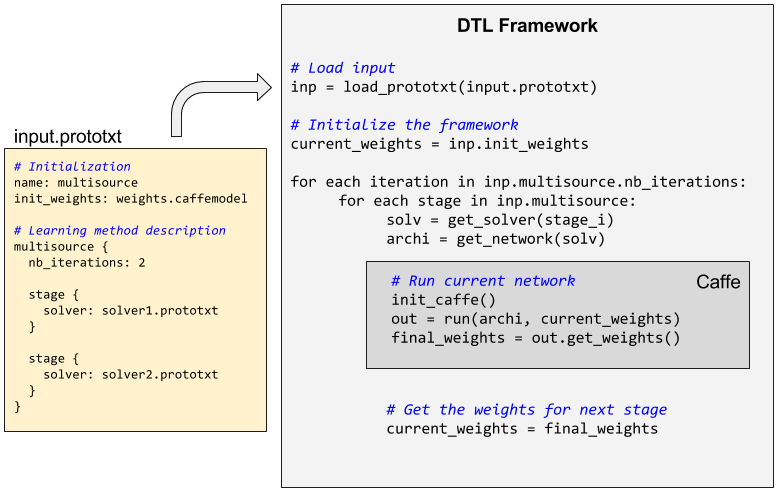
\includegraphics[width=\linewidth,center]{images/part3/dtl_framework_architecture.png}
  \caption{Architecture of the Deep Transfer Learning framework}\textbf{
  \label{fig:part3:dtl_framework_architecture}}
\end{figure}


\subsection{The metrics used} \label{3:tools:metrics}
For evaluating efficiently the accuracy of a model, we need to define a good evaluation measure. In our case, we are interested by semantic segmentation (pixel-wise labelling), so there are actually a lot of metrics those already exist in that field. It is complicated to define if the algorithm has made a "good job" because all of them have different requirements and goals : some applications does not need a perfect segmentation (with a precise delineation of the contours), and so, some algorithms can be considered efficient if they segment the images into uneven blobs as long as they classify them well.

It exists some methods and, for most of them, we first need to compute the confusion matrix (error matrix) to visualize the performance of our algorithm. This matrix will typically represent the results, crossing the predicted image with the expected one. \\
Considering an algorithm segmenting an image $\mathcal{I}$ from the dataset $\mathcal{D}$ into $n_{cl}$ classes. It will produce an output image $\mathcal{I}_{out}$ that has to be as similar as possible to the given ground truth image $\mathcal{I}_{gt}$. The metrics should, then, evaluate the similarity between the expected result $\mathcal{I}_{gt}$ and the predicted result $\mathcal{I}_{out}$. \\
To do this, we need to compute the confusion matrix, a matrix of size $(n_{cl}$, $n_{cl})$ with, for each cell $\mathcal{C}_{ij}$, the number of pixels that belongs to class $i$ (in $\mathcal{I}_{gt}$) and that are predicted to belong to class $j$ (in $\mathcal{I}_{out}$). \\
So, for each cell of the matrix we get :
$$ \mathcal{C}_{ij} = \sum_{\mathcal{I} \in \mathcal{D}} |\ \{ z \in \mathcal{I}\ such\ that\ \mathcal{I}_{gt}(z) = i\ and\ \mathcal{I}_{out}(z) = j \}\ | $$
Using this matrix, we also can define some terms as following :
\begin{itemize}
\item Number of pixels \textbf{L}abelled to belong to class i : $ L_i = \sum_{j=1}^{n_{cl}} \mathcal{C}_{ij} $
\item Number of pixels \textbf{P}redicted to belong to class j : $ P_j = \sum_{i=1}^{n_{cl}} \mathcal{C}_{ij} $
\item Total number of pixels : $ nb_{pixels} = \sum_{i=1}^{n_{cl}} \sum_{j=1}^{n_{cl}} \mathcal{C}_{ij} $
\end{itemize}

Using the matrix $\mathcal{C}$, we can compute five different useful metrics :
\subsubsection{The Overall Pixel accuracy (pixel accuracy)}
The number of pixels correctly labelled in all the images divided by the total number of pixels in the dataset. It may be a wrong metric for datasets that have an irregular repartition of the classes along their images. Indeed, if the class 'tree' is mainly present in the dataset, and if the dataset is only able to detect trees, the pixel accuracy is going to be good (equal to the percentage of trees in the dataset).
$$ pixel\_accuracy = \frac{\sum_{i=1}^{n_{cl}} \mathcal{C}_{ii}}{nb_{pixels}} $$
\subsubsection{The mean of the Per-Class accuracies (mean accuracy)}
The mean of the percentage of pixels well-labelled for all the classes over the images of the dataset. This metric resolve the problem of the imbalanced classes, because we do the percentage of pixels well-labelled for each class : it is class-dependant. On the other hand, with this metric, we may have some problem if one class is wrongly classified. For example, if the architecture is able to detect all the objects, except one which is a bit more difficult, the lack of performance in that class will seriously	 down-scale the mean accuracy.
$$ mean\_accuracy = \frac{1}{n_{cl}} \sum_{i=1}^{n_{cl}} \frac{\mathcal{C}_{ii}}{P_j} $$
\subsubsection{The Jaccard Index (the Jaccard similarity coefficient)}
The average of the intersections divided by the union of the labelled segments for each class, also called the Intersection over Union (IU). Concretely, if we have two sets $\mathcal{A}$ and $\mathcal{B}$, the IU would be $\mathcal{IU}(\mathcal{A}, \mathcal{B}) = \frac{|\mathcal{A} \cap \mathcal{B}|}{|\mathcal{A} \cup \mathcal{B}|} = \frac{|\mathcal{A} \cap \mathcal{B}|}{|\mathcal{A}| + |\mathcal{B}| - |\mathcal{A} \cap \mathcal{B}|}$. \\
Considering $\mathcal{A}$ the ground truth images, and $\mathcal{B}$ the segmented ones, we now can translate the formula into :
$$ \mathcal{IU} = \frac{\mathcal{C}_{ii}}{P_j + L_i - \mathcal{C}_{ii}} $$
And conclude that :
$$ mean\_iu = \frac{1}{n_{cl}} \sum_{i=1	}^{n_{cl}} \mathcal{IU}_i $$
This metric is, nowadays, the most used metric in semantic segmentation. \\
But it remains two problems with it : indeed, it is computed according to the amount of pixels, so then, it does not really take in consideration the exactness of the segmentation. Moreover, it is doing the mean of all the IUs, that can be a drawback if the accuracy is imbalanced between the classes.
\subsubsection{The frequency weighted IU}
Proposed by~\cite{LONG15} is a simple variant of the Mean IU, but it corrects the problem of the imbalanced classes by doing a weighted average of the classes, considering their proportion in the ground truth. Looking to the above $\mathcal{IU}_i$, it can be computed the following way :
$$ freq\_weighted\_iu = \frac{1}{nb_{pixels}} \sum_{i=1}^{n_{cl}} ( \mathcal{IU}_i L_i ) $$
\subsubsection{The Trimap metric}
An alternative metric have been proposed by Kohli et al.~\cite{KOHL09} for evaluating the segmentation around object boundaries. This model is a variant of the IU metric, but it is done only for selected pixels those are within a narrow band (called 'trimap') following the delineations of the classes. The advantage of this metric is that it adds the exactness notion, and also that we can compute few variants of it (depending on the width of the trimap). With a small width, the exactness notion is more significant, but we can not ensure anymore the global accuracy of the segmentation because it will ignore important objects information. On the other hand, if it is too large, we will have results similar to the IU measure.

It is also important to consider that all these metrics are dataset-based, which means that the measures are only done on the whole dataset. Csurka et al.~\cite{CSUR13} proposed to explore the per-class metrics. Indeed, an architecture can be really efficient on some images, but quite bad on some others with more difficult characteristics (luminosity, sharpness, ...). Then, the per-image score can be plotted in a histogram, and display which images are wrongly segmented. The main problem considering this, is that an image often does not have all the classes in it. Considering it, we can not apply the previous metrics anymore, because they all depend on the number of classes. Then, we have a computation a bit more complicated, because the ground truth and the predicted image may have different classes (due to mislabelling). The solution proposed by Csurka et al. consists in doing the per-image metrics the same way as for the whole dataset, but by considering only the classes that are present in both images (ground truth and predicted), even if some of them are mislabelled.



\section{The setups descriptions} \label{3:setups}
\begin{description}
\item[Problematic] Build a Deep Learning architecture able to provide, as fast as possible, an accurate segmentation of drone-derived data (aerial views).
\end{description}
Considering our problematic we can divide it into four main problems :
\begin{itemize}
\item "an accurate segmentation" ; we have to keep an eye on the accuracy of the system. We do this using the metrics previously described in section~\ref{3:tools:metrics}.
\item "as fast as possible" ; it means that we have to consider the time needed for the computation of each image.
\item "drone-derived data" ; we only work on small datasets, so we can imagine some pre-processing operations to extend it.
\item "Deep Learning architecture" ; we have few different architectures, we have to decide which one is the best one in our case
\end{itemize}

Considering this, we divided the research section into five main setups. All of them aim to find the best characteristic for each dimension of the learning. Also, we are going to test this final characteristics five times, to ensure its reproducibility.

\addcontentsline{toc}{subsection}{Setup 1. Find a way to process large images}
\subsection*{Setup 1. Find a way to process large images}
One problem with our datasets is the size of their images (respectively 4608x3456 and 3840x2160 for the Swiss and Okutama datasets). They are really large and cannot be processed like this. Usually, considering the capacity of recent GPUs and the architecture of the networks, it is common to process images of size 500x500.

In our case, we used two different operations : resizing and cropping. We tried different combinations. \\
About the Swiss dataset, it seems that the network was able to process images of size 576x432 (or less), so we can do few manipulations : resizing by 8, resizing by 4 and do a 2x2 cropping, resizing by 2 and do a 4x4 cropping, and a 8x8 cropping. \\
About the Okutama dataset, it seems that the network was able to process images of size 960x540 (or less), so we can do the following manipulations : resizing by 4, resizing by 2 and do a 2x2 cropping or do a 4x4 cropping.

These tests are done to find the best resolution to use for each dataset (to define if it is better to reduce the level of precision (resizing) or to reduce the size of our images (cropping)). Finally, when this level of precision is defined, we will also try another configuration that, intuitively, should be better : a random cropping (of a given size) on the dataset reduced to the best resolution.

Finding the best way to process large images is a main priority because all the following experiments would respect it. We did all these tests using one single architecture (FCN-32-ResNet-152), for 100.000 iterations, without transfer learning. The table~\ref{part3:setup1} resumes these trainings.

\rowcolors{2}{gray!25}{white}
\begin{table}[ht!]
  
  \begin{subtable}{\textwidth}
    \centering
    \begin{tabular}{cccccc}
    \rowcolor{gray!50}
    \toprule
    \textbf{Training set} & \textbf{Validation set} & \textbf{Resize} & \textbf{Crop} & \textbf{Final size}\\
    \midrule
    Swiss (80\%)     & Swiss (20\%)       & 8           & 1x1         & 576x432		 \\
	Swiss (80\%)     & Swiss (20\%)       & 4           & 2x2         & 576x432		 \\
	Swiss (80\%)     & Swiss (20\%)       & 2           & 4x4         & 576x432		 \\
	Swiss (80\%)     & Swiss (20\%)       & 1           & 8x8         & 576x432		 \\
    \midrule
	Okutama (80\%)   & Okutama (20\%)     & 4           & 1x1         & 960x540		 \\
	Okutama (80\%)   & Okutama (20\%)     & 2           & 2x2         & 960x540		 \\
	Okutama (80\%)   & Okutama (20\%)     & 1           & 4x4         & 960x540		 \\
    \bottomrule
    \end{tabular}%
    \caption{Experiments for the setup 1 - Resolution}
    \label{part3:setup1:resolution}
  \end{subtable}
  
  
  \begin{subtable}{\textwidth}
    \centering
    \begin{tabular}{rcccccc}
    \rowcolor{gray!50}
    \toprule
    \textbf{Training set} & \textbf{Validation set} & \textbf{Resize} & \textbf{Crop} & \textbf{Final size}\\
    \midrule
	Swiss (80\%)     & Swiss (20\%)       & best           & random         & 512x512		 \\
    \midrule
	Okutama (80\%)   & Okutama (20\%)     & best           & random         & 512x512			 \\
	Okutama (80\%)   & Okutama (20\%)     & best           & random         & 960x540			 \\
    \bottomrule
    \end{tabular}%
    \caption{Experiments for the setup 1 - Random cropping}
    \label{part3:setup1:randomcrop}
  \end{subtable}
  
  \caption{Setup 1}
  \label{part3:setup1}
\end{table}%


\addcontentsline{toc}{subsection}{Setup 2. Compare different models}
\subsection*{Setup 2. Compare different models}
Also, we have many models to test in our new datasets. As we saw in part~\ref{1:comparison}, the main models to try are SegNet, FCN-32-16-8, FCN-32-ResNet-50-101-152 and FCN-16-ResNet-50-101-152. Also, we can try all of them with the CRF end-to-end extension. All of these architectures should be tested on the Swiss dataset, considering the same sets (training / validation) as for the setup 1, and also for 100.000 iterations. Also, we would use the \textit{ad-hoc} way to process large images selected in the setup 1 ; it was a bit less efficient than the generic one, but much more faster to compute. For architecture comparison, we do not need to use the best pre-processing method. The final experiments for the Swiss dataset are resumed in the table~\ref{part3:setup2}, and the similarity between both datasets permits us to admit that the best architecture for one of them would also be the best for the other one.

\rowcolors{2}{gray!25}{white}
\begin{table}[ht!]
  \centering
  
  \begin{tabular}{rcccccc}
  \rowcolor{gray!50}
  \toprule
  \textbf{Architecture used} & \textbf{Pre-processing} \\
  \midrule
  SegNet    & see setup 1 (\textit{ad-hoc} method) \\
  FCN-32    & see setup 1 (\textit{ad-hoc} method) \\
  FCN-32-16    & see setup 1 (\textit{ad-hoc} method) \\
  FCN-32-16-8    & see setup 1 (\textit{ad-hoc} method) \\
  FCN-32-ResNet-50    & see setup 1 (\textit{ad-hoc} method) \\
  FCN-32-ResNet-101    & see setup 1 (\textit{ad-hoc} method) \\
  FCN-32-ResNet-152    & see setup 1 (\textit{ad-hoc} method) \\
  FCN-16-ResNet-50    & see setup 1 (\textit{ad-hoc} method) \\
  FCN-16-ResNet-101    & see setup 1 (\textit{ad-hoc} method) \\
  FCN-16-ResNet-152    & see setup 1 (\textit{ad-hoc} method) \\
  \bottomrule
  \end{tabular}%
  \caption{Experiments for the setup 2, done on the Swiss dataset}
  \label{part3:setup2}
\end{table}%


\addcontentsline{toc}{subsection}{Setup 3. Effects of Data Augmentation}
\subsection*{Setup 3. Effects of Data Augmentation}
Considering that we have very small datasets, we can try to improve the accuracy of our model by doing data augmentation, that means that we used same images as before, but also some variants of them, to improve the global size of the dataset. It consists in, while loading one image from the dataset, chose with 50\% of chances if we want to use this one, or a variant of it. This method adds some processing time (during the training phase) but permits to avoid a too heavy dataset. We decided to use four existing methods and their combinations.
\begin{itemize}
\item \textbf{Mirror :} While loading an image, we have 50\% chances to do a flip operation on it (horizontal or vertical, same probability). Considering our datasets, these kind of flips are coherent because we are processing aerial views, so they do not depend on orientation, and are flippable.
\item \textbf{Jittering operation :} This operation consists in selecting a random pixel in a small window (of a given size) and to apply it to the whole window. For example, for a jittering of 2, it would select one random pixel included in the top-left 2x2 pixels, and apply it to all of the four pixels. It is doing the same for the whole image.
\item \textbf{Noise injection :} This operation adds some noise to the image : it generates an array (similar size as the image) with values between 0 and 50, and adds these values to the real image, creating a noise effect.
\item \textbf{Random crop :} We define a crop size (such as 200x300), and it would crop randomly a part of the image. The given size of the crop should be big enough to still capture some objects characteristics.
\end{itemize}
The table~\ref{part3:setup3} resumes all the experiments to do for this setup. All of these were done with the \textit{ad hoc} pre-processing method defined in setup 1, because the random cropping is a bit more heavy to compute, and would have considerably increased the training time, moreover considering that we want to replicate our experiments. We tried all of them on both dataset, considering that the efficiency of the data augmentation is related to the images it contains.

\rowcolors{2}{gray!25}{white}
\begin{table}[ht!]
  \centering
  
  \begin{tabular}{rcccccc}
  \rowcolor{gray!50}
  \toprule
  \textbf{Data augmentation} & \textbf{Architecture} & \textbf{Pre-processing} \\
  \midrule
  None    & see setup 2       & see setup 1 (\textit{ad-hoc} method) \\
  Mirror    & see setup 2       & see setup 1 (\textit{ad-hoc} method) \\
  Jittering (2x2)    & see setup 2       & see setup 1 (\textit{ad-hoc} method) \\
  Noise    & see setup 2       & see setup 1 (\textit{ad-hoc} method) \\
  \bottomrule
  \end{tabular}%
  
  \caption{Experiments for the setup 3, for one dataset}
  \label{part3:setup3}
\end{table}%


\addcontentsline{toc}{subsection}{Setup 4. Deep Transfer Learning Methods}
\subsection*{Setup 4. Deep Transfer Learning Methods} \label{3:setups:4}
The fourth setup is going to be done for testing the Deep Transfer Learning methods. Indeed, we have two quite different datasets (Swiss and Okutama) and one of them is also divided into two similar locations (Okutama - close to the baseball field, or to the highschool). Considering these datasets, we can try to improve our results by using the multi-source method. The main goal is to improve a training with an other one from a different dataset. The table~\ref{part3:setup4} resumes the experiments of this setup, we also consider that all of them are done with trainings of 50.000 iterations, for three cycles, that means that we are going to train the architecture with the source dataset, then we finetune it with the target dataset, and reiterate this operation three times. Also, we are going to use the pre-processing method selected on setup 1, the architecture selected on setup 2, using the best data augmentation method found in setup 3.
\todo{+ compare with témoin = oku + swiss all at once}

\rowcolors{2}{gray!25}{white}
\begin{table}[ht!]
  \centering
  
  \begin{tabular}{rcccccc}
  \rowcolor{gray!50}
  \toprule
  \textbf{Training set} & \textbf{Transfer set} & \textbf{Validation set} \\
  \midrule
  Okutama (baseball)		& None			& Okutama (school)	\\
  Okutama (baseball)		& Swiss (80\%)	& Okutama (school)	\\
  Okutama (baseball)		& None			& Swiss (20\%)		\\
  Okutama (baseball)		& Swiss (80\%)	& Swiss (20\%)		\\
  \midrule
  Okutama (school)		& None     		& Okutama (baseball) \\
  Okutama (school)    	& Swiss (80\%)  & Okutama (baseball) \\
  Okutama (school)    	& None     		& Swiss (20\%) 		\\
  Okutama (school)    	& Swiss (80\%)  & Swiss (20\%) 		\\
  \midrule
  Okutama (80\%)    		& None     		& Okutama (20\%)		\\
  Okutama (80\%)    		& Swiss (80\%)  & Okutama (20\%) 	\\
  Okutama (80\%)    		& None     		& Swiss (20\%) 		\\
  Okutama (80\%)    		& Swiss (80\%)	& Swiss (20\%) 		\\
  \bottomrule
  \end{tabular}%
  
  \caption{Experiments for the setup 4}
  \label{part3:setup4}
\end{table}%


\addcontentsline{toc}{subsection}{Setup 5. Ensembles and model compression}
\subsection*{Setup 5. Ensembles and model compression}
In this section, we consider the method of the Ensembles, proposed by Dietterich~\cite{DIET00} that consists in running multiple architectures and, then, merging their results by averaging them (usually using a Bayesian averaging). This method already proves its efficiency~\cite{MARM16} and permits to build a more reliable segmentation (if two different networks segment a pixel the same way, it improves the probability that this pixel is segmented the good way). The averaging method can differ, three methods are mainly used :
\begin{itemize}
\item Majority voting : each pixel votes for a class, the winning one would be used for the final segmentation.
\item Average raw output : we simply average the outputs, for each pixels. It works only for linear classes.
\item Average class probabilities : we average the probabilities of each class for each pixel and, then, select the best one as usual.
\end{itemize}

This method requires a higher computational cost. Indeed, to build an average of the two networks, we need to compute the results of both of them, so it would, obviously, takes twice as much time.

Considering this con, we also had a look to the Distillation method, proposed by Hinton et al.~\cite{HINT15}, that consists in a compression method specialized for neural network. It actually alters a bit the accuracy, but permits to reduce an architecture into a smaller, compressed one. Usually, this method is used for improving the processing time of a single algorithm, but we thought that it also may be able to compress an ensemble of two architectures (as previously built) into a single one.

In this part, few ensemble methods can be tested, we listed the most interested ones in the table~\ref{part3:setup5}. All of these experiments have been done using the random cropping defined in setup 1 and the data augmentation method defined in setup 3.

\rowcolors{2}{gray!25}{white}
\begin{table}[ht!]
  \centering
  
  \begin{tabular}{rcccccc}
  \rowcolor{gray!50}
  \toprule
  \textbf{Name} & \textbf{Archi 1} & \textbf{Archi 2} & \textbf{Training set} \\
  \midrule
  1 & FCN-32-ResNet-50 & FCN-32-ResNet-152 & Okutama (80\%) \\
  2 & FCN-16-ResNet-50 & FCN-16-ResNet-152 & Okutama (80\%) \\
  3 & 1 & 2 & Okutama (80\%) \\
  4 & 3 & FCN-8 & Okutama (80\%) \\
  \bottomrule
  \end{tabular}%
  \caption{Experiments for the setup 5}
  \label{part3:setup5}
\end{table}%

